% -------------------------------------------------
\documentclass[12pt]{article}
\usepackage[utf8]{inputenc}
\usepackage{graphicx}
\graphicspath{ {./images/} }
\renewcommand{\baselinestretch}{1}
\usepackage[margin=1in]{geometry}
\usepackage[T1]{fontenc}
\usepackage{array}
\usepackage{caption}
\usepackage{float}
\usepackage{subcaption}
\usepackage{parskip} % paragraph separation
\usepackage{amssymb} % math symbols
\usepackage{amsmath}
\usepackage{amsfonts}
\usepackage[english]{babel}
\usepackage[sorting=none]{biblatex}
\addbibresource{FullRef.bib} %Imports bibliography 
\usepackage{csquotes}
\usepackage[title]{appendix}
\usepackage{hyperref}
\usepackage{verbatim}
\usepackage{longtable}

\usepackage{amsthm}
\theoremstyle{plain}
\newtheorem{theorem}{Theorem}
\newtheorem{lemma}{Lemma}
\theoremstyle{definition}
\newtheorem{definition}{Definition}
\theoremstyle{remark}
\newtheorem*{remark}{Remark}

% -------------------------------------------------
%                   Start here
% -------------------------------------------------
\begin{document}
\thispagestyle{empty}
\begin{center}
{\Huge Shuffling Algorithms and Users’ Perceptions of Randomness, with Application to Streamed Music

\bigskip
\bigskip


\bigskip
\bigskip

\huge Anbang Du\\
\vspace{5pt}
\huge Warwick ID: 1700247\\
\bigskip
\bigskip
\bigskip


\LARGE Supervised by Dr.Julia Brettschneider}
\end{center}
\vfill

\begin{center}
{\Large
Department of Statistics\\
University of Warwick\\
Coventry CV4 7AL\\
United Kingdom\\
\medskip

Email: a.du.3@warwick.ac.uk \\
\medskip

6 May 2021 }
\end{center}
\bigskip

\newpage

% -------------------------------------------------
% abstract and acknowledgement


% -------------------------------------------------

\tableofcontents

\clearpage

% -------------------------------------------------

\section{Introduction}


\section{Shuffling Theory}
\subsection{Top in at Random Shuffle}

Image there is a deck of n cards. \textit{Top in at random}\cite[Example~1 on \pno~333]{1.1} shuffle refers to the process of randomly inserting the top card of a deck into the deck. A sharp estimate for the number of times the deck needed to be shuffled until it is random is $nlog(n)$. Before going into a rigorous construction of this idea, let us look at the intuition behind it. If some cards get inserted under the original bottom card, we call these cards well-shuffled because all relative orders of these cards are equally likely. Then, the whole deck is well-shuffled as long as the bottom card comes to the top and gets inserted into the deck. 

Recall that a geometric distribution is a distribution of number of trails needed to get the first success in repeated Bernoulli trails. Accordingly, the number of trails/time taken for a top card to go under the original bottom card is clearly geometric, with a probability of success $\frac{k}{n}$, where $n$ refers to the total number of cards and $k$ the current position of the original bottom card. This is simply because the top card has k places to go under the original bottom card. Also, note that the expected value for a geometric random variable is the reciprocal of the probability of success, i.e. $E(X)=\frac{1}{p}$. Therefore, total time taken to perfectly shuffle a deck of cards is approximately $$T = \frac{n}{1} + \frac{n}{2} + \cdots + \frac{n}{n-1} + \frac{n}{n} \approx nlog(n).$$

In order to establish this claim rigorously, we first model a step distribution for the \textit{top in at random} shuffle. Consider a permutation group $S_n$, which contains all possible permutations of $n$ objects. Then, $\{Q(\pi):\pi \in S_n\}$ is a step distribution for different steps $\pi$. Note that no matter where the top card goes in each step, the probability for every single step stays uniform, i.e.  $$Q(1)=Q(2,1)=\cdots=Q(n-1,\cdots,1)=Q(n,\cdots,1)=\frac{1}{n}$$ where $(i,i-1,\cdots,1)$ is a cycle notation representing a permutation $\pi$ mapping the first card to the $i$th position and other cards move accordingly. This enables us to further model the multiple-step distribution using convolution\cite[\pno~334]{1.1}: $$Q^k(g)=QQ^{k-1}(g)=\sum_{h\in S_n}Q(h)Q^{k-1}(gh^{-1})$$
This means, say $k=2$, at the first step we have a permutation $h$, and next we have $gh^{-1}$, and we sum up all possible $h$. To clarify, $gh^{-1}$ is a single permutation with the effect of $h$ being removed from $g$, such that we can achieve a combined permutation of $g$ finally after 2 steps.

At this stage we can model the current position of a deck after $k$ shuffles. However, we may want to ask how far is the current distribution of cards from the perfect shuffle? To answer this, we define the variation distance, which is a distance metric measuring the distance between 2 distributions, as following\cite[\pno~335]{1.1}:
\begin{equation*}
\begin{split}
    \|Q_1-Q_2\|&\triangleq \frac{1}{2}\sum_{g\in G}|Q_1(g)-Q_2(g)|\\
    &=\max_{A\subset G}|Q_1(A)-Q_2(A)|
\end{split}
\end{equation*}
where $Q_1(A)=\sum_{g\in A}Q_1(g)$.

In our context, we let $d(k)=\big\|Q^k-U\big\|$ be the variation distance between the $k$-step distribution and the uniform distribution. In other words, $d(k)$ measures how far $k$ repeated shuffles is from perfectly shuffle. As you can see here we use the uniform distribution to model the perfect shuffle. Then, we have the following theorem.

\begin{theorem} \cite[Theorem~1 on \pno~335]{1.1}
For the top in at random shuffle,\\
(a) $d(n\log n + cn)\leq e^{-c}$; all $c\geq 0$, $n \geq 2$.\\
(b) $d(n\log n - c_nn)\rightarrow 1$ as $n\rightarrow \infty$; all $c_n \rightarrow \infty.$
\end{theorem}

\begin{remark}
What this theorem really says is $nlogn$ shuffles can approximately get the deck perfectly shuffled. However, this idea is expressed in a tricky way. We bound the variation distance of more shuffles (than $nlogn$) from above by 0 and bound the variation distance of less shuffles from below by 1. This means any more shuffles than $nlogn$ will result in a variation distance close to 0, where any less shuffles than $nlogn$ will result in a variation distance nearly one. Therefore, it gives an idea that $nlogn$ shuffles are enough in an asymptotic sense.
\end{remark}

\begin{remark}
After above set-ups, we claim that there exists $k_0=nlog(n)$ such that $d(k_0+O(k_0))\approx0$ and $d(k_0-O(k_0))\approx1$.\footnote{For the big $O$ notation: when $x\in R$ in $f(x)$ goes to infinity, the term of $f(x)$ which grows at the fastest rate is kept. By getting rid of any constant this term has, i.e. $c$ in $cg(x)$, we call the resulting term $g(x)$. Then, $f(x)=O(g(x))$ if and only if there exists $M \in R_+$, such that  $|f(x)|\leq Mg(x)$ for large enough $x$.  } 
\end{remark}

Let me introduce stopping time and strong uniform time as they will be used in the proof of the theorem.
\begin{definition}
  Let $Q$ be a distribution on a permutation group $S_n$, which contains all possible permutations of $n$ objects, and $\{X_k\}_{k\geq1}$ the associated random walk (position after k steps). $T$ is a \textit{stopping time} with respect to the random walk if $\{T=j\}$ is completely determined by at most the total information known up to time $j$, i.e. $(X_0,\cdots,X_j)$.
\end{definition}

\begin{definition}  
\textit{Strong uniform time} is a stopping time $T$ such that $P(X_k=g,T=k)$ is independent of $g$, for all $k<\infty$, $g\in S_n$. 
\end{definition}

\begin{lemma}\cite[Remark~(i) on \pno~336]{1.1}
The following two conditions are equivalent to the above definition. 
\begin{itemize}
    \item $P(X_k=g|T=k)=\frac{1}{|S_n|},g\in S_n$.
    \item $P(X_k=g|T\leq k)=\frac{1}{|S_n|},g\in S_n$.
\end{itemize}
\end{lemma}

\begin{remark}
This lemma basically says when we know the the random walk stops at $k$ or before $k$, the probability of being in any positions at time $k$ are uniform, i.e. any possible permutations/arrangement of cards at time $k$ are equally likely. Therefore, the idea is that we use strong uniform time to model the instant $T$ where the deck of cards is well shuffled. 
\end{remark}
Furthermore, we need two more lemmas to prove Theorem 1.

\begin{lemma}\cite[Lemma~1 on \pno~336]{1.1}
Let $Q$ be a probability distribution on a finite group $G$, let $T$ be a strong uniform time for $Q$. Then, $$d(k)\triangleq \|Q^k-U\|\leq P(T>k),\forall k \geq 0.$$
\end{lemma} 

\begin{proof}
For any $A\subset G$,
\begin{equation*}
\begin{split}
Q^k(A)&=P(X_k\in A)\\
&=P(X_k\in A,T\leq k)+P(X_k\in A,T>k)\\
&=\sum_{j\leq k} P(X_k\in A,T=j)+P(X_k\in A,T>k)\\
&=\sum_{j\leq k} P(X_k\in A|T=j)P(T=j)+P(X_k\in A|T>k)P(T>k)\\
&=\sum_{j\leq k} U(A)P(T=j)+P(X_k\in A|T>k)P(T>k)\\
&=U(A)\sum_{j\leq k} P(T=j)+P(X_k\in A|T>k)P(T>k)\\
&=U(A)(1-P(T>k))+P(X_k\in A|T>k)P(T>k)\\
&=U(A)+P(T>k)(P(X_k\in A|T>k)-U(A))
\end{split}
\end{equation*}

In the fifth line of the equation, we used the fact that $P(X_k\in A|T=j)=U(A)$ as mentioned in the previous lemma. In the seventh line, we used the fact that $$\sum_{j\leq k}P(T=j)=P(T\leq k)=1-P(T> k).$$ The last line is simple algebra. Note that $P(X_k\in A|T>k)\neq U(A)$ because the probability after $k$ shuffles has not yet been uniform when $T>k$. Then it follows that $$\{P(X_k\in A|T>k)-U(A)\}\in (-1,1)\setminus \{0\},$$
which gives $$|Q^k(A)-U(A)|\leq P[T>k], \forall A\subset G$$
\end{proof}

\begin{lemma}\cite[Lemma~2 on \pno~337]{1.1}
Sample from an urn with $n$ balls uniformly with replacement. Denote $V$ to be the required number of draws for each of $n$ balls being drawn at least once. Then,
$$P[V>n\log n+cn]\leq e^{-c};c\geq0,n\geq1.$$
\end{lemma} 

\begin{proof}
Let $m=n\log n+cn$, and denote the event $A_b$=\{ball b has not yet been drawn in first m draws\}. Then, 
\begin{equation*}
\begin{split}
    P(V>m)&=P(A_1\cup A_2\cup \cdots \cup A_n)\\
    &=P(\bigcup_{b=1}^{n}A_b)\\
    &\leq \sum_{b=1}^{n}P(A_b)\\
    &=n(1-\frac{1}{n})^m\\
    &\leq n\exp{(-\frac{m}{n})}\\
    &=e^{-c}
\end{split}
\end{equation*}

The first line is simply due to the very definition of the event $A_b$: since $V>m$, to draw each ball once we need more than $m$ draws, thus within $m$ draws there exists one ball or some balls that have not been drawn once yet. Therefore, it is equivalent to the union of all $A_b$. In the third line, we used the union bound to get the inequality. The $n$ in $n(1-\frac{1}{n})^m$ in the fourth line represents there are $n$ balls in the urn; while $P(A_b)=(1-\frac{1}{n})^m$ is the probability of ball $b$ not been drawn in the first $m$ draws.

In the fifth line, the inequality is derived using the fact that $(1+x)\leq e^x, \forall x \in R$ with $m>1$. The last equality is derived as follows:\[
n\exp{(-\frac{m}{n})}=\exp{(\log n-\frac{m}{n})},
\]
and $\log n-\frac{m}{n}=-c$ since we have set $m=n\log n+cn$ at the beginning of the proof.
\end{proof}

\textbf{Proof of Theorem 1(a)}
\begin{proof}
Recall $T$ is the first time the original bottom card gets to the top and being inserted in the deck, and it is a strong uniform time. The idea is to show it has the same distribution as $V$ in Lemma 2, and then apply both lemmas to get the result.
\begin{equation}
    T=T_1+(T_2-T_1)+\cdots+(T-T_{n-1})
\end{equation}
Here we decompose $T$ as above, and note that $T_i$ is the instant the $i$th card is placed under the original bottom card. When there are exactly $i$ cards got inserted below the original bottom card, i.e. we are standing at time $T_i$, 
\begin{gather}
P(\text{\it{current top card is inserted below the original bottom card}})=\frac{i+1}{n}\nonumber\\
\Longrightarrow P(T_{i+1}-T_i=j)=(\frac{i+1}{n})(1-\frac{i+1}{n})^{j-1}
\end{gather}


,since the random variable $T_{i+1}-T_i$ has a geometric distribution with $P(success)=\frac{i+1}{n}$. Then, the random variable $V$ as described in Lemma 2 can be decomposed as:
\begin{equation}
    V=V_1+(V_2-V_1)+\cdots+(V-V_{n-1})
\end{equation}
Note $V_i$ is the number of draws taken when $i$ distinct ball(s) has been drawn at least once. Therefore, when $i$ distinct ball(s) has been drawn,
\begin{gather}
P(\text{\it{a new ball is drawn in a draw}})=\frac{n-i}{n}\nonumber\\
\Longrightarrow P(V_{i+1}-V_i=j)=(\frac{n-i}{n})(1-\frac{n-i}{n})^{j-1}
\end{gather}
,since the random variable $V_{i+1}-V_i$ has a geometric distribution with $P(success)=\frac{n-i}{n}$. Clearly, $V_{n-i}-V_{n-i-1}$ and $T_{i+1}-T_i$ have the same distributions, i.e.
$$P(V_{n-i}-V_{n-i-1}=j)=P(T_{i+1}-T_i=j).$$
In (1), each of $T_{i+1}-T_i$ are independent; in (3), each of $V_{i+1}-V_i$ are also independent. Then, their respective sums, $T$ and $V$, have the same distribution. By lemma 1 and 2, $$ d(n\log n+cn)\leq  P(T>n\log n+cn)\leq e^{-c},\forall c\geq0,n\geq1$$
\end{proof}

\textbf{Proof of Theorem 1(b)}
\begin{proof}
With $j$ fixed, let $A_j$ be the set of arrangement of cards such that the original bottom $j$ cards remain in their original relative order. For instance, $A_{20}$ is the set containing all events with the relative order of bottom 20 cards remains unchanged after shuffling. An important implication here is that an event will no longer belong to $A_{20}$ if in this event the $20th$ card from bottom gets to the top and then inserted into the original 19 bottom cards, because it surely breaks the original order of them. Besides, we note that $$U(A_j)=\frac{1}{j!}$$

Let $k=k(n)=n\log n-c_nn,c_n\rightarrow\infty.$ Since $$d(k)\triangleq \|Q^k-U\|=
    \max_{A\subset G}|Q^k(A)-U(A)|\geq \max_{j}|Q^k(A_j)-U(A_j)|,$$
and we want to show $d(k)\rightarrow 1$ as $n\rightarrow \infty$, it suffices to show $\max_{j}|Q^k(A_j)-U(A_j)|\rightarrow 1$. In fact, we will prove $Q^k(A_j)\rightarrow 1$ at first. 

We claim $P(T-T_{j-1}>k)\leq Q^k(A_j)\leq 1$. If this is true, and if $P(T-T_{j-1}>k)\longrightarrow 1$, then the result follows by the sandwich lemma. The second inequality is trivial, and we will look at the first one. Recall $T$ is the time taken that the original bottom card comes to the top and gets inserted in the deck. Then, $T-T_{j-1}$ takes out the time for inserting $j-1$ cards under the bottom card from $T$. It can be equivalently seen as the time taken for the card initially $j$th from bottom to come to top and get inserted. To justify, $$T-T_{j-1}=(T_j-T_{j-1})+(T_{j+1}-T{j})+\cdots+(T-T_{n-1}),$$ 
which clearly shows while we are inserting each top cards, we are moving the original bottom card, who is currently at position $j$, up to the top and finally insert it to the deck.  

Therefore, the event $\{T-T_{j-1}>k\}$ means the $j$th card from bottom initially have not been inserted yet, and as explained at the beginning, the original relative order of the bottom $j$ cards remains the same up to time $k$, which implies $$\{T-T_{j-1}>k\}\subseteq A_j,$$
which proves the first inequality. 

Now we show $P(T-T_{j-1}>k)\rightarrow 1$, which is the same as $P(T-T_{j-1}\leq k)\rightarrow 0$. To prove this we need the Chebyshev's Inequality:
$$P(|X-E(X)|\geq s)\leq \frac{V(X)}{s^2},s\geq 0$$
By (2) and properties of geometric distribution,
\begin{gather*}
    E(T_{i+1}-T_i)=\frac{1}{p}=\frac{n}{i+1}\\
    V(T_{i+1}-T_i)=\frac{1-p}{p^2}=\frac{1-\frac{i+1}{n}}{(\frac{i+1}{n})^2}
\end{gather*}
Then we have,
\begin{equation*}
\begin{split}
    E(T-T_{j})&=\sum_{i=j}^{n-1}E(T_{i+1}-T_i)\\
    &=\sum_{i=j}^{n-1}\frac{n}{i+1}\\
    &\approx n\int_{i=j}^{n-1}\frac{1}{x+1}dx\\
    &=n\log n-n\log (j+1)\\
    &=n\log n+O(n)
\end{split}
\end{equation*}
\begin{equation*}
    \begin{split}
    V(T-T_{j})&=\sum_{i=j}^{n-1}V(T_{i+1}-T_i)\\
    &=\sum_{i=j}^{n-1}(\frac{n}{i+1})^2(1-\frac{i+1}{n})\\
    &\approx O(n^2)
    \end{split}
\end{equation*}

\begin{equation*}
    \begin{split}
    P(T-T_{j-1}\leq k)
    &=P(T-T_{j-1}\leq n\log n -c_nn)\\
    &=P[T-T_{j-1}-(n\log n+O(n))\leq n\log n -c_nn-(n\log n+O(n))]\\
    &=P[T-T_{j-1}-E(T-T_{j-1})\leq -c_nn-O(n)]\\
    &\leq P[|T-T_{j-1}-E(T-T_{j-1})|\leq c_nn+O(n)]\\
    &\leq \frac{V(T-T_{j-1})}{c_nn^2+O(n)}\\
    &=\frac{O(n^2)}{c_nn^2+O(n)}\\
    &=\frac{\frac{O(n^2)}{n^2}}{c_n+\frac{O(n)}{n^2}}\longrightarrow 0
    \end{split}
\end{equation*}
Thus $P(T-T_{j-1}>k)\rightarrow 1$, by the sandwich lemma, $Q^k(A_j)\rightarrow 1$. Since $U(A_j)$ is very small when $j$ is large, we have $$d(k)\triangleq \|Q^k-U\| \geq \max_{j}|Q^k(A_j)-U(A_j)|\rightarrow 1, n\rightarrow \infty$$
\end{proof}

\newpage
\subsection{Riffle Shuffle}
A riffle shuffle is to cut off the deck into 2 roughly equal part and riffle them together. Imagine that we number a deck from 1 to 52, then we cut off the deck into 2 parts, say one part has 1-24, the other has 25-52. Now if we riffle them together, we shall see 1 or 2 rising sequences as a result. Note that 1 rising sequence refers to the case that the part 1-24 is riffled to the top of the part 25-52, though I have to admit it is a pretty bad riffle shuffle. Therefore, a riffle shuffle can be seen as a permutation with 1 or 2 rising sequences. 1 rising sequence corresponds to the identity permutation.

If c cards are cut off from top of a n-card deck, there are $\binom{n}{c}$ possible shuffles. This is because a riffle shuffle is essentially choosing $c$ places out of $n$ places. Next if $c$ is no longer fixed, the total number of possible riffle shuffles is \[1+\sum_{c=0}^n \left(\binom{n}{c}-1\right)=2^n-n.\]

To see this, we note first $c$ takes value from 0 to $n$. However, no matter what value does $c$ take, or no matter how many cards we cut off initially, the 1-increasing-sequence case (identity permutation) of riffle shuffle is unique and we should only count it once. For example, when $c=2$, the 1-increasing-sequence case is 1-52; however, it is still the case for any other $c$.

Gilbert, Shannon and Reeds have built the following model \cite[\pno~343]{1.1} for random riffle shuffle.

\begin{theorem}
Select an integer $c \in\{0,\cdots,n\}$ according to a binomial distribution with probability \[P[C=c]=\binom{n}{c}\left(\frac{1}{2}\right)^c\left(\frac{1}{2}\right)^{n-c}.\]
Cut off $c$ cards and hold in left hand, $n-c$ in right hand. Drop the cards from a given hand with the probability proportional to packet. Then, the chance that a card is initially dropped from left hand is $\frac{c}{n}$; and then, the chance that the next card is dropped from the left hand is $\frac{c-1}{n-1}$, and so on. This models a riffle shuffle.
\end{theorem}

\begin{lemma}\cite[Lemma~7 on \pno~343]{1.1}
The following two descriptions are equivalent to the description in the above theorem.
\begin{itemize}
    \item Cut an $n$-card deck with respect to a binomial distribution with $n$ and $p=\frac{1}{2}$. If c cards are cut off, pick one of the $\binom{n}{c}$ possible shuffles uniformly.
    \item An inverse shuffle $\pi^{-1}$ can be generated with same probability as in statement 2. Label the back of each card with the result of an independent, fair coin toss, {0,1}. Take those labelled 0 and place them on the top of the deck, without changing the relative order for each group of 1 or 0. 
\end{itemize}
\end{lemma}

\begin{proof}
Denote the three descriptions \textbf{1, 2, 3} respectively.\\
$\mathbf{1 \iff 2} :$ The probability of the riffling process described in \textbf{1} is $$\frac{(c)(c-1)(c-2)\cdots(2)(1)\cdot(n-c)(n-c-1)(n-c-2)\cdots(2)(1)}{(n)(n-1)(n-2)\cdots(2)(1)}=\frac{c!(n-c)!}{n!}$$
The probability of uniformly picking one of the $\binom{n}{c}$ possible shuffles in \textbf{2} is 
$$\binom{n}{c}^{-1}=\frac{c!(n-c)!}{n!}.$$ 
$\mathbf{2 \iff 3} :$ Binary labelling chooses a binomially distributed number of zeros. Then, all possible placements of zeros are equally likely, with probability $\binom{n}{c}^{-1}$.
\end{proof}


\begin{remark}\cite[Lemma~8 on \pno~343]{1.1}
\textbf{3} implies $$\big\|Q(g)-U\big\|=\big\|Q(T^{-1}(g))-U\big\|,$$ where $Q$ a probability on a finite group $G$, $T:G\rightarrow G$, $U$ the uniform distribution and $g\in G$.
\end{remark}

In fact, when we repeat the process described in \textbf{3}, i.e. the inverse shuffle, we are able to record this process in a binary matrix \cite[344]{1.1} (each entry of the matrix is a binary string). The construction of such a binary matrix can help us derive the time for the perfect shuffle.

\[\begin{matrix}
a\;101 & \;\;\;\;\;\;\;\;\;\; b\;001 & \;b\;001 & \;d\;010\\
b\;001 & \;\;\;\;\;\;\;\;\;\; d\;010 & \;a\;101 & \;c\;110\\
c\;110 & \;\;\;\;\;\;\;\;\;\; a\;101 & \;d\;010 & \;b\;001\\
d\;010 & \;\;\;\;\;\;\;\;\;\; c\;110 & \;c\;110 & \;a\;101
\end{matrix}\]

On the very left hand side, the \textbf{column 0} represents the starting point of inverse shuffles. You may notice each card $a,b,c,d$ is assigned a binary string, which indicates their behaviour at each shuffle. Entry $(i,j)$ of the matrix represents which card is at position $i$ after $j$ th shuffle, i.e. card $d$ at the entry $(3,1)$ means after 3 shuffles $d$ is on the top of the deck.

The behaviour of cards can be described as follows (from left to right): 
\begin{itemize}
    \item At \textbf{column 0}, observe the first entries of all rows are 1, 0, 1, 0. Recall for a inverse shuffle we are to gather all 0's and place them on top of the 1's. Therefore, we have 0, 0, 1, 1 in the first entries of rows in \textbf{column 1}.
    
    \item Now we look at the second entries of rows in \textbf{column 1}. Again, since the binary labelling of 0's and 1's has been done, we take all 0's and place them on top of the 1's, giving us the 0, 0, 1, 1 in \textbf{column 2}. 
    
    \item Then, look at the third entries of rows in \textbf{column 2}, where the binary labelling has been done. Following the same logic, we arrive at the third entries of rows, 0, 0, 1, 1, in \textbf{column 3}.
\end{itemize}

If we look at this binary matrix from right to left, we can easily find out that as we proceed from one column to another, a riffle shuffle is performed. For example, at \textbf{column 3}, a binomial cut has been performed, i.e. the third entries of rows are 0, 0, 1, 1. Then, we riffle them together to proceed to \textbf{column 2}, which has the third entries of 1, 1, 0, 0. To proceed further, look at the second entries of rows and repeat the procedure. In this direction, the deck is sorted alphabetically.

Why the inverse shuffle is important? As mentioned above, we can derive the time for the perfect shuffle with the help of it: using, again, the strong uniform time.

\begin{lemma}\cite[Lemma~9 on \pno~344]{1.1}
If $T$ is the first time that the binary matrix formed by inverse shuffling has distinct rows, then $T$ is a strong uniform time.
\end{lemma} 

\textbf{Distinct} rows in a column is used to describe the state of perfectly shuffled. Note that rows in a column are \textbf{distinct} means there does not exists increasing sequences of cards. The intuition of this goes back to the very beginning of this section, where we have stated that 
\begin{itemize}
    \item a riffle shuffle creates at most 2 rising sequences.
\end{itemize}
Based on this, 2 riffle shuffles create 4 rising sequences at most, 3 create 8 at most, etc. Then, it makes sense to see that the number of riffle shuffles is enough if performing it no longer generates more rising sequences (existing increasing sequences of cards have length of 1). Equivalently, a deck of cards is perfectly riffle-shuffled when there does not exists increasing sequences of cards. Then,
\begin{itemize}
    \item $T$ is a strong uniform time if the deck of cards is perfectly riffle-shuffled at $T$.
\end{itemize}

\begin{proof}
When the rows are distinct, the joint distribution of any permutation of the deck is invariant, i.e. probability of any permutation is constant. Thus, at time $T$, all $n!$ permutations of cards are equally likely.
\end{proof}

The following theorem gives an upper bound for the variation distance between $k$-step riffle shuffle and the uniform distribution.

\begin{theorem}\cite[Theorem~5 on \pno~344]{1.1}
Let $Q$ be a Gilbert-Shannon-Reeds probability distribution defined in Theorem 2. Then,
\[   \big\|Q^k-U\big\| \leq P(T > k) = 1 - \prod_{i=1}^{n-1}(1-\frac{i}{2^k}).  \]
\end{theorem}

\begin{proof}
The inequality follows directly from lemma 1. For the equality, consider dropping $n$ balls into $2^k$ boxes. The strong uniform time $T$ in this context is the time that no two balls are in the same box.  Accordingly, $\{T>k\}$ is the event that there exists boxes that contain more than 1 ball. $\{T\leq k\}$ is the event that there are no two or more balls in the same box. 

Clearly, $$P\{T\leq k\}=\prod_{i=1}^{n-1}(1-\frac{i}{2^k}).$$
\end{proof}
This upper bound can be explicitly calculated by inputting values of $n$ and $k$. For instance\cite[344]{1.1}, when $n=52$, and $k=10, 11, 12, 13, 14$, the values of the upper bound are 0.73, 0.48, 0.28, 0.15, 0.08 respectively. Furthermore, if $n$ balls are regarded as $n$ people, and $2^k$ boxes as $2^k$ birthdays, the example becomes a famous birthday problem.

\newpage
\subsection{Perception of Randomness}
Since one of our aims is to explore the difference between the actual randomness and the perceived randomness, we will discuss some examples of misperception of randomness in this section.

Instead of judgement tasks, production tasks used to be the main focus in earlier study for perception of randomness. Still, it is the majority nowadays. However, in our project the emphasis lies on the judgement task as it is much more relevant to our objectives. In this section, I will mainly explain the cognitive biases in people's perception of randomness and exemplify them with some judgement studies.

The study from Wagenaar\cite[434]{1.2} suggested the existence of negative recency effect and local representativeness effect in some earlier production tasks. Alternation bias that appeared in human-produced binary strings refers to too many alternations among events, and local representativeness is over-balancing of events over short regions\cite[434]{1.2}. Since they are essentially cognitive biases, they should have counterparts in a judgement task. In Falk's study\cite[434]{1.2}, she found either in a judgement task or a production task, the preferred alternation rate for randomness was 0.6; similarly, from Wagenaar\cite[435]{1.2}, "sequences with conditional probabilities [of repetition] around 0.4 were judged as most random".

A real-world based example for the alternation bias of randomness is the \textit{"hot hand" phenomenon} in basketball games. Basketball fans believe that when a player makes a steak of hits, he is in a state of \textit{hot hands}, and under such state, the probability of next hit is higher than if he did not make previous hits. However, the data of shooting record\cite[437]{1.2} forming the basis of such belief provided no evidence for sequential dependency for streak shooting. It rather demonstrated that any steak made by any player was merely clumping of random events generated by a random device with probability of that player's hit rate\cite[437]{1.2}. From this example, we can easily find that people expect more alternations than it should be for a random process.

A famous example for the local representativeness effect is the gambler's fallacy. It is gambler's reputed belief that when one has bad luck for a long time, the chance of having good luck immediately is much higher than usual. In other words, people expect a balancing for the frequencies of events over short period of time. This was practically demonstrated in Gold and Hester's\cite[437]{1.2} study. In this study, the subjects exhibited self-contradicting patterns, demonstrating that the gambler's fallacy is indeed a fallacy: in a sequence of coin tosses, subjects believed the next outcome would be \textit{head} after seeing a sequence of consecutive tails; on the other hand, if the coin was replaced by another one before the target toss, or was held for a while before the target toss, subjects changed their belief of the next outcome to \textit{tail}. 


\newpage




\section{Randomness in Playlists}
In the previous section, we have seen how the distribution of a deck of cards can be modelled, and how to construct the top in at random shuffle and riffle shuffle; moreover, we are clear now why randomness is described by the uniform distribution. Apart from this, in the view of various psychology papers, we notice that some perceived "patterned" event turned out to be clumping of random events. This is called the misperception of randomness.

In music streaming applications like Spotify, if you click shuffle-play in a playlist, you will get a shuffled playlist that you feels random but not random actually\cite{2.0}. This is due to the avoidance of clumping of random event as mentioned above. In this section, I would like to see that, in a sample of user-created music playlists, are the songs randomly ordered, or are they patterned in some ways? 

\subsection{Million Playlist Dataset}
The dataset used in this section is the Million Playlist Dataset (MPD) introduced in the RecSys Challenge 2018\cite{2.2}, sponsored by Spotify. The MPD consists of 1,000,000 playlists created by US Spotify users between January 2010 and October 2017, with over 2 million unique songs by nearly 300,000 artists. It was created by sampling (with randomisation) from more than 4 billion public playlists on Spotify, with manual filtration regarding to playlists quality. Besides, the dataset has some dithering and fictitious tracks added to them. This means the dataset does not represent the true distribution of playlists on Spotify.\cite{2.1} 

In September 2020, Spotify released an identical challenge with the same MPD, and it was the continuation of the RecSys Challenge 2018. The motivation of such challenge is playlists research. As noted in this blog\cite{2.1}, Spotify would like to learn the nature of playlists and then be able to better capture users' taste through recommending songs and playlists. To be more specific, given a set of playlist features, participants' systems shall generate a list of recommended tracks that can be added to that playlist, i.e. automatic playlist continuation.

I will use this dataset to see how the songs in the playlists distributed and whether or not we can detect any patterns in their distributions.

\subsection{Data Extraction}
Since the MPD is huge, I selected one slice of it to work on, i.e. slice 6000-6999. The data is "raw", as you can see that a playlist (truncated to save space) takes the following form\cite{2.1}: 
\begin{verbatim}
    {
        "name": "musical",
        "collaborative": "false",
        "pid": 5,
        "modified_at": 1493424000,
        "num_albums": 7,
        "num_tracks": 12,
        "num_followers": 1,
        "num_edits": 2,
        "duration_ms": 2657366,
        "num_artists": 6,
        "tracks": [
            {
                "pos": 0,
                "artist_name": "Degiheugi",
                "track_uri": "spotify:track:7vqa3sDmtEaVJ2gcvxtRID",
                "artist_uri": "spotify:artist:3V2paBXEoZIAhfZRJmo2jL",
                "track_name": "Finalement",
                "album_uri": "spotify:album:2KrRMJ9z7Xjoz1Az4O6UML",
                "duration_ms": 166264,
                "album_name": "Dancing Chords and Fireflies"
            },
            // 10 tracks omitted
            {
                "pos": 11,
                "artist_name": "Mo' Horizons",
                "track_uri": "spotify:track:7iwx00eBzeSSSy6xfESyWN",
                "artist_uri": "spotify:artist:3tuX54dqgS8LsGUvNzgrpP",
                "track_name": "Fever 99\u00b0",
                "album_uri": "spotify:album:2Fg1t2tyOSGWkVYHlFfXVf",
                "duration_ms": 364320,
                "album_name": "Come Touch The Sun"
            }
        ],

    }
\end{verbatim}
That is why we need to extract the information we need for a good analysis of randomness of playlists. Note that the whole data extraction process was performed using the Jupyter Notebook and the code can be found in the Appendix section. The whole procedure can be broken into these parts: 

\begin{itemize}
    \item Download the Spotify Million Playlist Dataset.
    \item Since the complete dataset is huge, I selected a slice of data (\textit{mpd.slice.6000-6999.json}) to work on. This dataset contains nearly a thousand playlists.
    \item Using the Jupyter Notebook, connect to the Spotify’s Web API where I can access the information I need for a good analysis. 
    \item Write a function to extract the audio features, i.e. danceability, acousticness, etc., for a single song.
    \item Let this function loop through every song in every playlists in the dataset.
    \item Write the final output of audio features to a \textit{csv.} file.
\end{itemize}

Besides, let me explain what does different music features mean. These definitions are based on \cite{2.3}.
\begin{itemize}
    \item \textbf{Danceability:} Danceability describes how suitable a track is for dancing based on a combination of musical elements including tempo, rhythm stability, beat strength, and overall regularity. A value of 0.0 is least danceable and 1.0 is most danceable.
    \item \textbf{Energy:} Energy is a measure from 0.0 to 1.0 and represents a perceptual measure of intensity and activity. Typically, energetic tracks feel fast, loud, and noisy. 
    \item \textbf{Loudness:} The overall loudness of a track in decibels (dB). Loudness values are averaged across the entire track and are useful for comparing relative loudness of tracks. Loudness is the quality of a sound that is the primary psychological correlate of physical strength (amplitude). Values typical range between -60 and 0 db.
    \item \textbf{Mode:} Mode indicates the modality (major or minor) of a track, the type of scale from which its melodic content is derived. Major is represented by 1 and minor is 0.
    \item \textbf{Speechiness:} Speechiness detects the presence of spoken words in a track. The more exclusively speech-like the recording (e.g. talk show, audio book, poetry), the closer to 1.0 the attribute value. Values above 0.66 describe tracks that are probably made entirely of spoken words. Values between 0.33 and 0.66 describe tracks that may contain both music and speech, either in sections or layered, including such cases as rap music. Values below 0.33 most likely represent music and other non-speech-like tracks.
    \item \textbf{Acousticness:} A confidence measure from 0.0 to 1.0 of whether the track is acoustic. 1.0 represents high confidence the track is acoustic.
    \item \textbf{Instrumentalness:} Predicts whether a track contains no vocals. “Ooh” and “aah” sounds are treated as instrumental in this context. Rap or spoken word tracks are clearly “vocal”. The closer the instrumentalness value is to 1.0, the greater likelihood the track contains no vocal content. Values above 0.5 are intended to represent instrumental tracks, but confidence is higher as the value approaches 1.0.
    \item \textbf{Liveness:} Detects the presence of an audience in the recording. Higher liveness values represent an increased probability that the track was performed live. A value above 0.8 provides strong likelihood that the track is live.
    \item \textbf{Valence:} A measure from 0.0 to 1.0 describing the musical positiveness conveyed by a track. Tracks with high valence sound more positive (e.g. happy, cheerful, euphoric), while tracks with low valence sound more negative (e.g. sad, depressed, angry).
    \item \textbf{Tempo:} The overall estimated tempo of a track in beats per minute (BPM). In musical terminology, tempo is the speed or pace of a given piece and derives directly from the average beat duration.
    \item \textbf{Duration in ms:} The duration of the track in milliseconds.
\end{itemize}

\newpage
\subsection{Exploratory Data Analysis}
After the data extraction, we now have a well-prepared data where we can start to do some analysis. In this section I will give a general look of the selected slice of data. This include the density plot for each audio features, and the box plot for the distribution of first several songs. 

\begin{figure}[htp]
    \centering
    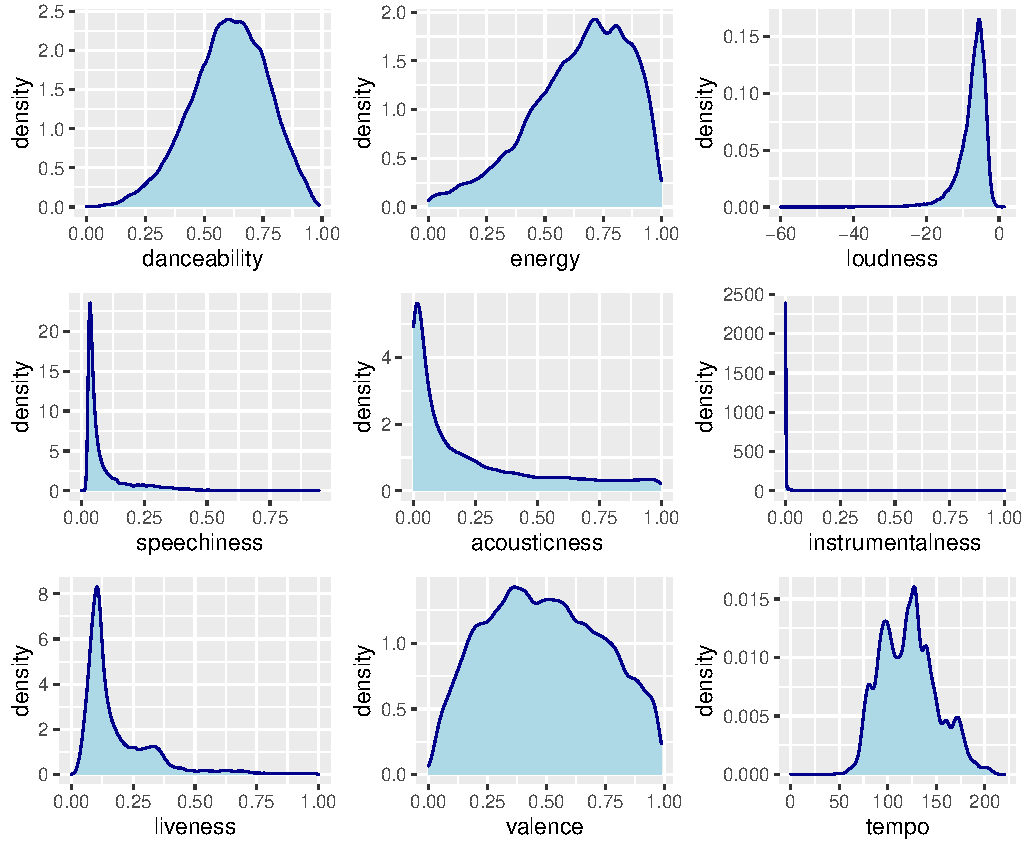
\includegraphics[width=\textwidth]{Images/density.pdf}
    \caption{\textbf{Density Plots of the Variables.} This is a density plot for 9 audio features in our extracted playlist data (slice 6000-6999 in MPD). For danceability, energy, they are close to a normal density but with slight skewness. Some of them have very long tails and very concentrated distributions over very narrow regions, i.e. loudness, speechiness, liveness. An extreme example of such "concentration" would be instrumentalness, since all the mass is on a tiny neighbourhood at 0. For tempo, it seems to have 2 peaks, one is around 99 and the other is about 126.}
    \label{fig:Density}
\end{figure}



After seeing how each of audio features are distributed, I wanted to see whether the distributions of the first several songs are different from the remaining songs/each other in all playlist in our data. This is interesting because if that is true, then this slice of MPD does have patterns in common; however, this cannot be realistic since the MPD was mainly created by sampling from a gigantic pool of playlists. This will be explained in detail in a while. Let us look at the following plots.

\begin{figure}[htp]
    \centering
    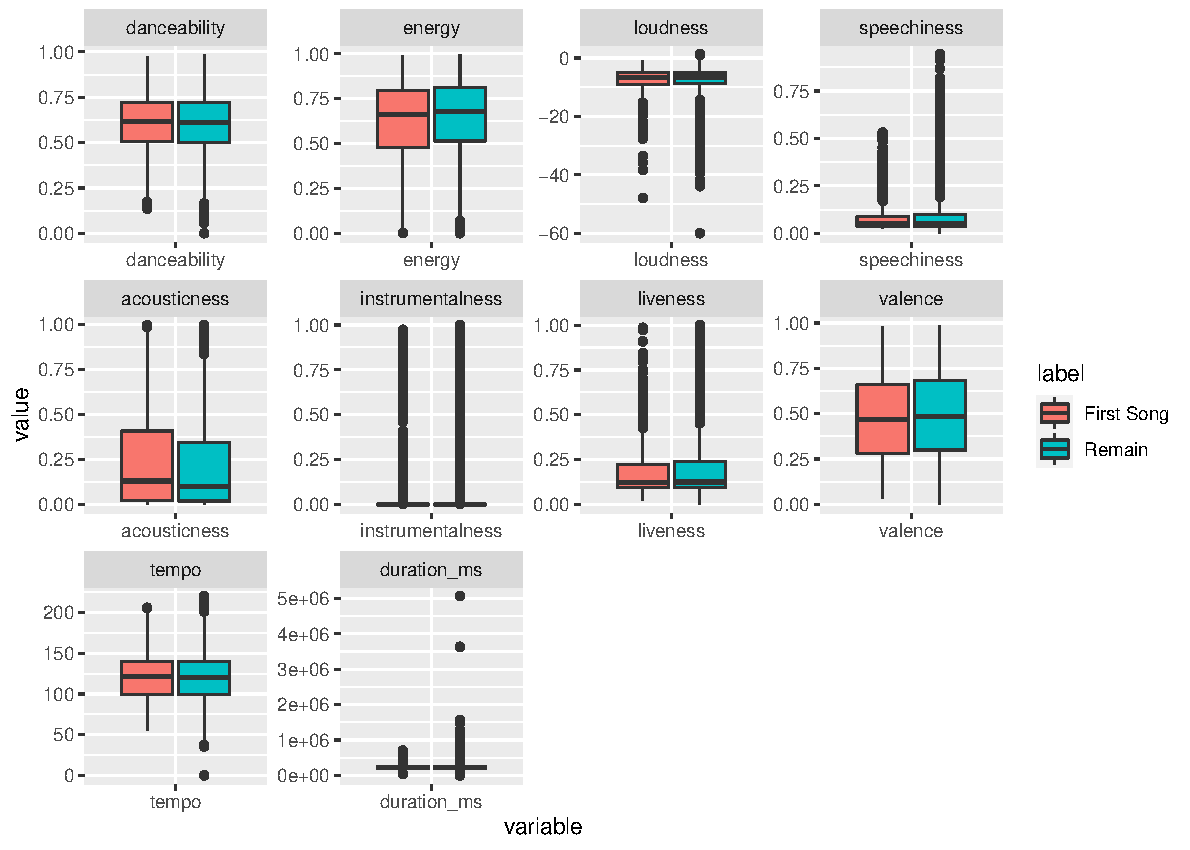
\includegraphics[width=\textwidth]{Images/1st.pdf}
    \caption{\textbf{Comparing the distribution of the first songs and the remaining songs in all playlists in our extracted data.} This is done by extracting the first songs in all playlists and store them in a new vector. Also store the remaining songs in all playlists in another vector. Then generate a boxplot between these two vectors. For all 10 variables, there is no significant difference between the two distributions.}
    \label{fig:1st}
\end{figure}

\begin{figure}[htp]
    \centering
    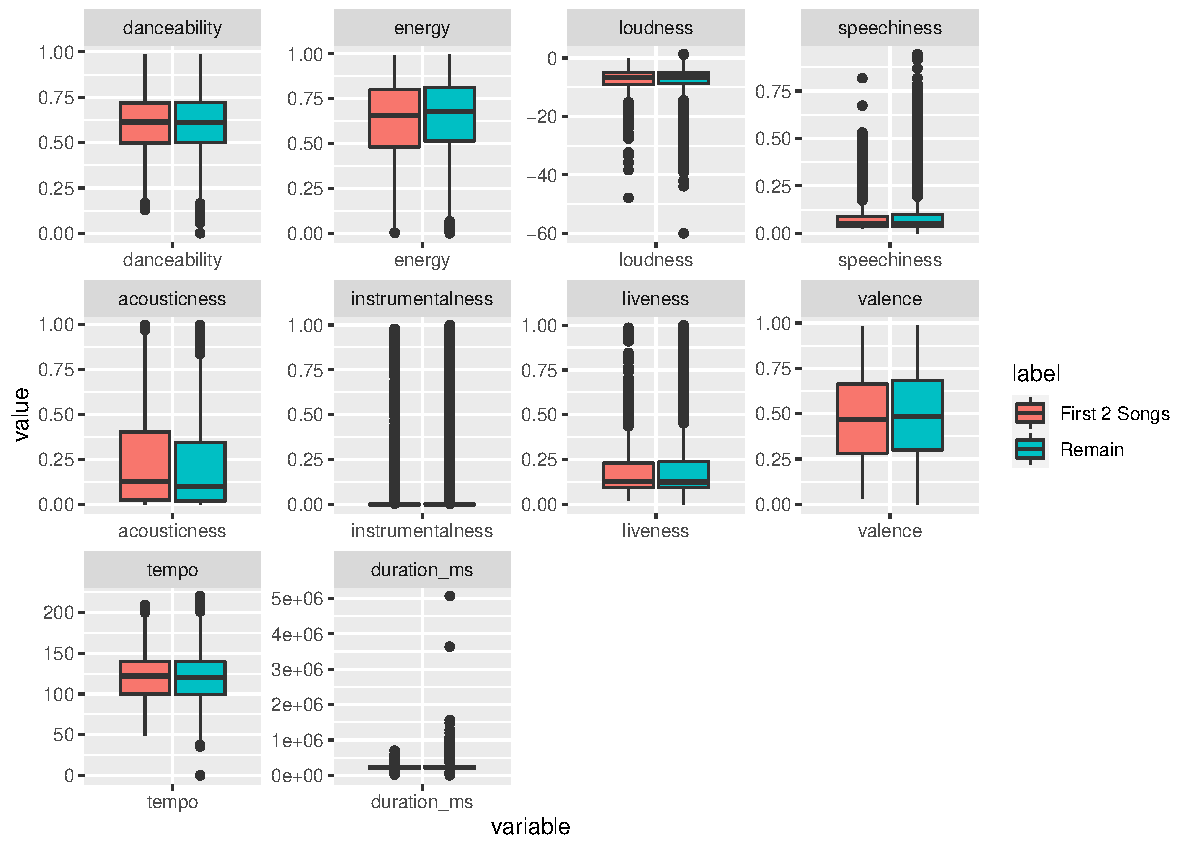
\includegraphics[width=\textwidth]{Images/1st2.pdf}
    \caption{\textbf{Comparing the distribution of the first two songs and the remaining songs in all playlists in our extracted data.} Similarly, there is no significant difference between the two distributions.}
    \label{fig:1st2}
\end{figure}

\begin{figure}[htp]
    \centering
    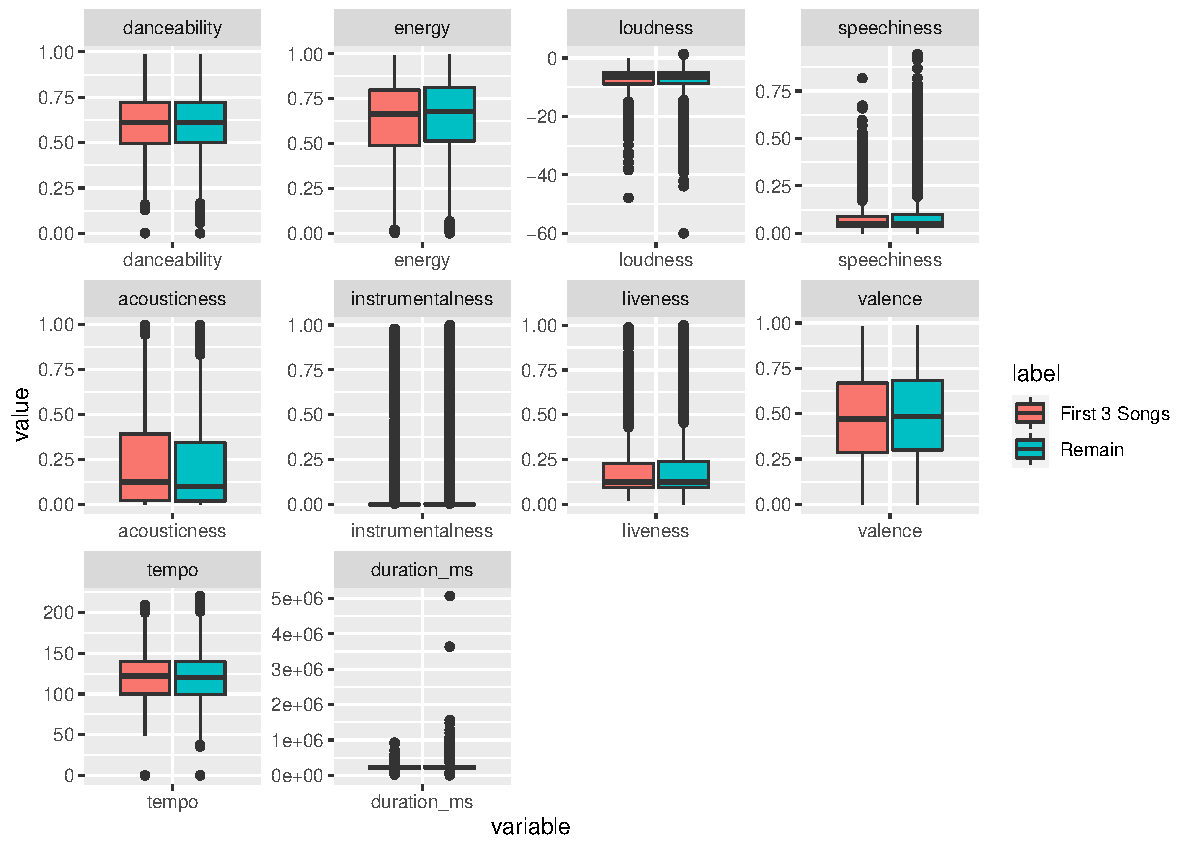
\includegraphics[width=\textwidth]{Images/1st3.pdf}
    \caption{\textbf{Comparing the distribution of the first three songs and the remaining songs in all playlists in our extracted data.} Again, there is no significant difference between the two distributions.}
    \label{fig:1st3}
\end{figure}

\newpage
\begin{figure}[h]
    \centering
    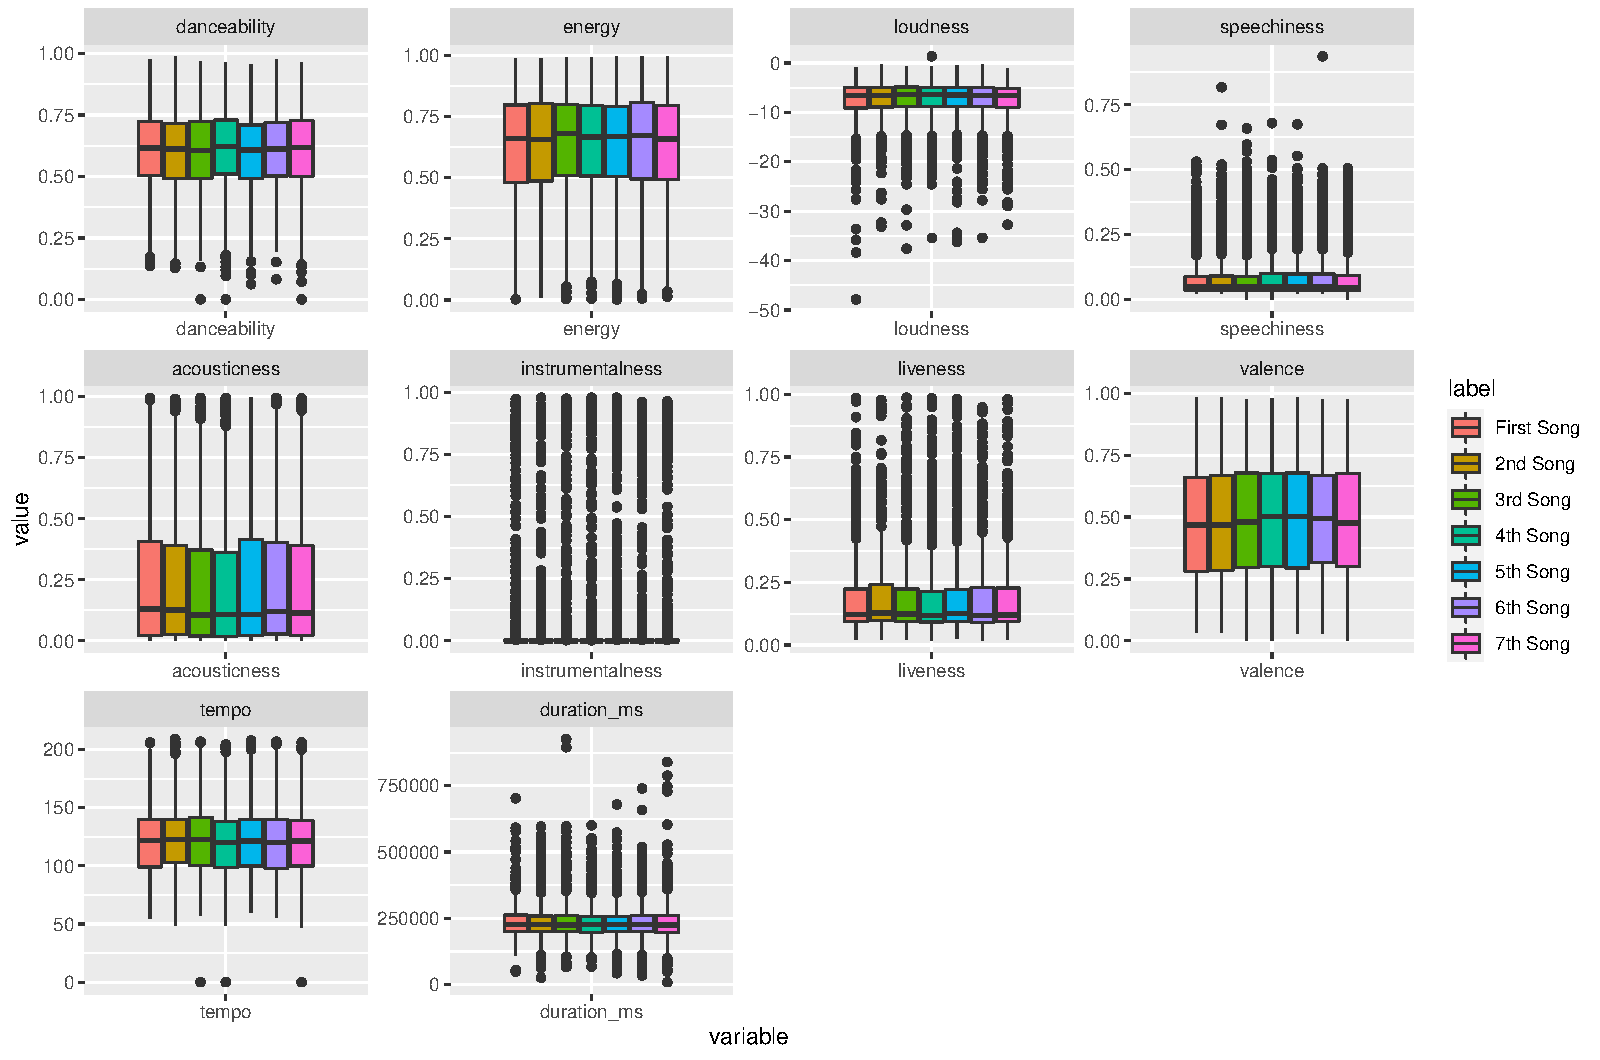
\includegraphics[width=\textwidth]{Images/1st7.pdf}
    \caption{\textbf{Distribution of the First 7 Songs.} Regardless of the remaining songs, we focused on the distributions of the first 7 songs. This gives a clearer picture that when we look at all 1000 playlists together, no patterns in any of the audio features can be observed.}
    \label{fig:1st7}
\end{figure}


The aim of these box plots is to see whether the distribution of the first several songs are different from remaining songs or each other. In fact, in this way one can hardly find any significant difference in the distributions. A simple example can clarify. Let us consider a distribution of a single variable speed/tempo of 1000 three-song-playlists. Suppose all 1000 playlists are created by one user who uses them in the gym and prefer an order of "fast song - slow song - fast song", then we can expect the distribution of the three songs to show a clear sign of non-randomness. However, the assumptions made here are rarely true in reality (so in our case), because all 1000 playlists cannot be made by only one person for only one purpose (different taste and different purpose). Thus, if one playlist has an order, say, "fast song - slow song - fast song", and another has "slow song - fast song - slow song", we would see nothing in their collective distribution since the non-randomness gets cancelled out. 

Overall, though non-randomness might exist in individual playlists, it cannot be captured in a comparison between the collective distributions of 1000 first songs, 1000 second songs, ..., etc, unless some strict, unrealistic assumptions are made. 

\newpage







\section{Runs Test}
Although we have not been able to find any evidence of non-randomness in the last section by comparing their distributions of first several songs, this leads to a more reliable direction of work: since we cannot capture the non-randomness in the collective distribution of the songs in playlists, we can instead examine them individually by looking at one playlist at a time. This lead us to the runs test\cite{3.5}.

\subsection{Concept}
 At first let me introduce some basic concept in the runs test.

\begin{itemize}
    \item \textbf{General idea:} we first convert a sequence of numerical values into a binary sequence using a threshold value, then we can use runs test to see whether the original sequence of number are randomly distributed above and below the threshold value.
\end{itemize}

From this idea we can see if we convert, say, danceability of a single playlist into a binary string, we are able to use the runs test to see whether or not the songs are randomly ordered in terms of danceability.

\begin{itemize}
    \item \textbf{Null Hypothesis:} the original sequence of number are randomly distributed above and below the threshold value.
    \item \textbf{Alternative Hypothesis:} the original sequence of number are not randomly distributed above and below the threshold value.
\end{itemize}

To apply the runs test, the hypothesis evaluated with the runs test is shown above, and the null hypothesis is randomness. Next I will define some fundamental terminologies in the runs test.

\begin{itemize}
    \item \textbf{Run:} a run is a sequence of consecutive numbers that are either all above or all below your threshold value, where the choice of how you divide your data is usually the mean or the median. 
    \item $\mathbf{n_1},\mathbf{n_2}$: the number of occurrence for each alternative in the binary string.
    \item $\mathbf N$: length of the sequence; also equal to $n_1+n_2$
\end{itemize}

\[\mathbf{\textbf{Series 1:}\;\;\;\;0\;0\;0\;1\;1\;0\;0\;1\;1\;1\;1\;1\;0\;0\;1}\]
\[\mathbf{\textbf{Series 2:}\;\;\;\;0\;0\;0\;0\;0\;1\;1\;1\;1\;1\;1\;1\;1\;1\;1}\]

For example, these are 2 sequence of numbers with $N=15$ that have already been converted into 2 binary strings according to some thresholds. Let us look at series 1: there are 6 runs, with $n_1=7,n_2=8$. Series 2: there are 2 runs, with $n_1=5,n_2=10$.

Furthermore, the runs test is a non-parametric test, because it evaluates categorical data, and we do not consider its distribution parameters in this case.

\newpage
\subsection{Theory}
Essentially, the runs test is performing a comparison between the observed number of runs and the expected number of runs. The null hypothesis of randomness is rejected when the total number of runs of A’s and B’s is too many or too few. 

\begin{itemize}
    \item When $N$ is small, the test statistic is exactly the total number of runs $R$. Thus, from the table of critical values of single sample runs test \cite[Table~A8]{3.4}, we can directly use $R$ to arrive at a conclusion on randomness. The table gives an "acceptable" range of $R$. If the observed $R$ falls outside of the range, being too many or too few, we reject the null hypothesis.
    \item When $N$ is big, i.e. $n_1,n_2>10$, the normal distribution can be employed to approximate the exact
    distribution of runs\cite{3.4}\cite{3.1}\cite{3.3}, with
    \begin{gather*}
      z=\frac{R-\mu_R}{\sigma_R}\\
      \mu_R=\frac{2n_1n_2}{n_1+n_2}+1\\
      \sigma_R=\sqrt{\frac{2n_1n_2(2n_1n_2-n_1-n_2)}{(n_1+n_2)^2(n_1+n_2-1)}}
    \end{gather*}
    \item Note that if we want to compute exact p values, we must calculate the following probabilities \cite{3.3}\cite{3.6}, i.e. the number of runs being even and odd respectively. And the last equation is how we calculate the p value. The $r$ in the last equation refers to the realisation of the random variable $R$.
    \begin{gather}
      P(R=2m)=\frac{2\binom{n_1-1}{m-1}\binom{n_2-1}{m-1}}{\binom{N}{n_1}}\\
      P(R=2m+1)=\frac{\binom{n_1-1
      }{m}\binom{n_2-1}{m-1}+\binom{n_2-1}{m} \binom{n_1-1}{m-1}}{\binom{N}{n_1}}\\
      P(|R-\mu_R|\ge|r-\mu_R|)=\sum_{i=2}^{\mu_R-|r-\mu_R|}P(R=i)+\sum_{i=\mu_R+|r-\mu_R|}^{2min(n_1,n_2)+1}P(R=i)
    \end{gather}
\end{itemize}

In fact, (7) is pretty straight forward. If we recall the fact that the p value is actually calculating the area of the tails or probability of the tail events, we can see this equation is doing exactly the same thing. the left hand side $P(|R-\mu_R|\ge|r-\mu_R|)$ is the probability that the number of runs $R$ is more far away from the mean than the current realisation $r$, while the right hand side calculated the area of the 2 tails. Note the lower bound of the left tail and the upper bound of the right tail are the minimum and maximum of $R$ respectively. The minimum $R$ for a binary string is 2, if we ignore the case $n_i=0$. The maximum $R$ is $2min(n_1,n_2)+1$, if $N$ is odd; an even $N$ does not need to add an extra run. 

\begin{itemize}
    \item (5) is the case when $R$ is even, (6) when $R$ is odd, $m$ taking values of 1, 2, 3, ... .
    \item The denominators in (5) and (6) are both $\binom{N}{n_1}$, i.e. the number of ways of placing $n_1$ in $N$ positions, and it can be regarded as the total number of permutations. 
    \item The numerators are then reasonably being the number of permutations that can result in $R$ runs.
    \item Imagine a binary sequence with $A$'s and $B$'s. For (5), since $R$ is even, if the sequence starts with $A$, then it must end with $B$, vice versa. This explains the "2" in the numerator. We will consider the case starting with $A$ ending with $B$, i.e. $$A\;\;\; \cdots \;\;\; B$$Ignoring the repetition of $B$, in order to get $2m$ runs, we want to place exactly one $B$ \textbf{after} $m-1$ places of $n_1-1$ $A$'s. $m-1$ is because we already have one $B$ fixed at the end, so we only need $m-1$ more runs of $B$. $n_1-1$ is because we are placing $B$ \textbf{after} $A$ and already one $B$ is fixed at the end. Therefore, we have $$\binom{n_1-1}{m-1}.$$ Now let us allow the repetition of $B$. The key point here is how each run of $B$ repeats purely depends on how $A$ divides them. So if ignoring the repetition of $A$'s and treating them as the spacers in $B$'s, we are counting the number of ways placing exactly one $A$ \textbf{before} $m-1$ places of $n_1-1$ $B$'s. $m-1$ is because, similarly, a run of $A$ is fixed and counted at the beginning, so only $m-1$ more runs of $A$ is needed. $n_2-1$ is because we are placing $A$ \textbf{before} $B$ and one $A$ is already fixed at the start. Therefore, we have $$\binom{n_2-1}{m-1}.$$
    \item For (6), since $R$ is odd, we will have either of below: $$A\;\;\; \cdots \;\;\; A$$
    $$B\;\;\; \cdots \;\;\; B$$ In the first case, ignoring the repetition of $B$, in order to get $2m-1$ runs, we should place exactly one $B$ \textbf{after} $m$ places of $n_1-1$ $A$'s. $n_1-1$ is because we are placing $B$ after (either after or before is okay, both will yield same result) $A$, so the $A$ fixed at the end is ignored. $m$ is because since we start and end with $A$, $A$ will have $m+1$ runs while $B$ will have $m$. Now allowing for repetition of $B$ and treat $A$ as the spacers, since there are 2 $A$'s fixed at the start and the end, $m+1-2=m-1$ more runs of $A$ is needed. Also, we are placing spacers of $A$ within $B$'s, we have $n_2-1$ positions to choose from in total. Therefore, we have $$\binom{n_1-1}{m}\binom{n_2-1}{m-1}.$$ Similarly in the second case, where the sequence starts and ends with $B$, we first ignore the repetition of $A$ and treat it as the spacers between $B$'s. How many more runs should our spacers $A$ contribute? Since $B$ has $m+1$ runs in this case, only $m$ runs needed from $A$. How many places can the spacers go? Within 2 $B$'s, there are $n_2-1$ spaces in total. Now allow for repetition of $A$, and treat $B$ as spacers within $A$'s. How many more runs should our spacers $B$ contribute? Since there is one at the beginning and one at the end, now we only have $m+1-2=m-1$ more runs needed from spacers $B$. How many places can the spacers go? Regardless of 2 $B$'s at 2 ends, we are essentially placing spacers $B$ within $A$'s, so we have $n_1-1$ spaces in total. Therefore, we have $$\binom{n_2-1}{m} \binom{n_1-1}{m-1}.$$
\end{itemize}


\newpage
\subsection{Application}
What we essentially want from the runs test is the $p$-value. It is the probability that the number of runs $R$ is at least as extreme as the observed number of runs $r$, conditional on $H_0$ being true. Also, as noted before, the $p$-value the probability of tail events, which is also equivalent to the area of the tail when we looking at the distribution of runs. Therefore, the smaller the $p$-value, the smaller the probability of the tail events, the stronger the evidence to reject the null hypothesis.

We need to be very cautious when we apply the runs test to our data, since
\begin{itemize}
    \item our dataset contains 997 playlists, and 8 music features/columns. 
    \item one of the music features, \textbf{tempo}, seems to have 2 peaks in its density plot.
\end{itemize}

The implication of the first bullet point not only involves a careful design of function in R, but also the fact that we will be performing thousands of runs test, which clearly associate with the multiple testing problem. I will discuss the multiple testing problem in chapter 5. In the remaining of this chapter, I will focus on the design of the desired function and also address the issue raised in the second bullet point. Some of the code will be included here for clarification purpose, but the complete version of the code can be found in the appendix.

What has already been done in the EDA section is locating the starting position (row number) of each playlist. I have arranged the positions in a vector called $ind1$, and used it to generate the plots in the EDA section. As you can see below, I used the function $lag$ to find the starting point of a new playlist, and then $ind1$ is defined to be positions of all first songs in the dataset.
\begin{verbatim}
    ind1 <- which(song$playlist_name != lag(song$playlist_name))
    ind1 <- c(1,ind1)
\end{verbatim}
Now we consider how to find the position of the last songs in each playlists. It turns out to be $ind1[i]-1$. However, if we run this for all $i=1, \cdots, 997$, we would miss the last playlist in the dataset. Thus, we create a vector $IND$ to overcome it. Now the final playlist is captured when $i=998$. 
\begin{verbatim}
    ind1[1]:(ind1[2]-1)
    ind1[2]:(ind1[3]-1)
    IND<-c(ind1,nrow(song)+1)
    IND[997]:(IND[998]-1)
\end{verbatim}
Then, after installing and load the package $randtests$ \cite{3.7}, we can write the desired function as $RT$. Note that the function $runs.test$ has a list of output and we just want its $p$-value. The threshold for the runs test can be the mean or median of the input vector.
\begin{verbatim}
    RT<-function(a){
     p<-rep(0,997)
     for (i in 1:997) {
       p[i]<-runs.test(a[IND[i]:(IND[i+1]-1)],
       threshold = mean(a[IND[i]:(IND[i+1]-1)]))$p.value
     }
     return(p)
    }
\end{verbatim}

\begin{verbatim}
    RT<-function(a){
     p<-rep(0,997)
     for (i in 1:997) {
       p[i]<-runs.test(a[IND[i]:(IND[i+1]-1)],
       threshold = median(a[IND[i]:(IND[i+1]-1)]))$p.value
     }
      return(p)
    }
\end{verbatim}
Now this function $RT$ allows me to perform runs test on each of the music feature/columns, in return giving me a vector of $p$-value for each column of the dataset. We name each of the vector in terms of their corresponding music features, and count how many $p$-value are significant, for $\alpha=0.05$.
\begin{verbatim}
    P.dance<-RT(song$danceability)
    nrow(as.data.frame(which(P.dance<0.05)))
    P.energy<-RT(song$energy)
    nrow(as.data.frame(which(P.energy<0.05)))
    P.loudness<-RT(song$loudness)
    nrow(as.data.frame(which(P.loudness<0.05)))
    P.speechiness<-RT(song$speechiness)
    nrow(as.data.frame(which(P.speechiness<0.05)))
    P.acousticness<-RT(song$acousticness)
    nrow(as.data.frame(which(P.acousticness<0.05)))
    P.liveness<-RT(song$liveness)
    nrow(as.data.frame(which(P.liveness<0.05)))
    P.valence<-RT(song$valence)
    nrow(as.data.frame(which(P.valence<0.05)))
\end{verbatim}

The count for the number of significant results after applying $RT$ (with threshold mean and median respectively) to each column of our dataset is given in the table below.
\begin{longtable}{|c|c|c|}
    \hline
     Audio Features & No. of Significant Results (mean) & No. of Significant result (median) \\
    \hline
     Danceability &129&125\\
     \hline
     Energy &156&152\\
     \hline
     Loudness &190&173\\
     \hline
     Speechiness &126&119\\
     \hline
     Acousticness &159&135\\
     \hline
     Liveness &76&52\\
     \hline
     Valence &110&118\\
    \hline
  \caption{\textbf{Number of significant observations for each audio features in the dataset after applying the runs test, with threshold being the mean and the median respectively.} The result shows, when we choose the mean to be the threshold for the runs test, the highest number of significant observations is in loudness, where 190 out of 997 playlists reported non-randomness; on the other hand, the lowest is in liveliness, where only 76 out of 997 reported non-randomness.If we set the threshold to be median, we would observe a generally similar outcome, with the highest count being 173 (loudness) and the lowest being 52 (liveliness). Notice neither of the 2 threshold had made the significant observations above $20\%$.}
  \label{table 1}
\end{longtable}

Note that we left the variable \textbf{tempo} in the dataset because it has more than one category (due to the fact that it has 2 peaks in its density plot) thus it cannot be input in $RT$, our ordinary runs test function. We will deal with it in the next section.


\newpage
\subsection{K-category extension of the runs test}
Let us address the issue for the column \textbf{tempo}, which has 2 peaks observed from the density plot. It seems inappropriate to convert it into a binary factor; instead, we could divide it into a three category variable using some thresholds. This introduces the k-category extension of the runs test\cite{3.4}\cite{3.3}.

\begin{itemize}
    \item \textbf{K-category extension of the runs test:} a runs test used on a categorical variable with more than 2 categories.
    \item $\mathbf{n_i}:$ number of observations in the $i$th category.
    \item $\mathbf N:$ sum of $n_i$ for all $i$.
    \item $\mathbf{\mu_R}:$ the expected number of runs,
    $$\mu_R=\frac{N(N+1)-\sum n_i^2}{N}$$
    \item $\mathbf{\sigma_R}:$ the expected standard deviation,
    \[\sigma_R=\sqrt{\frac{\sum n_i^2(\sum n_i^2+N(N+1))-2N\sum n_i^3-N^3}{N^2(N-1)}}\]
    \item \textbf{Test statistic:} the asymptotic $z$ statistic is computed from the observed number of runs and the above quantities, $$z=\frac{r-\mu_R}{\sigma_R}.$$
\end{itemize}

However, there is no readily available package for the K-category extension of the runs test. Therefore, I designed a new function based on the existing function $runs.test$ in the package $randtests$. Now I will introduce how I constructed this function step by step. Note that the codes included here are the key part of the whole function, and some of the unimportant code are excluded here. You can still find the complete code in the Appendix.

By looking at the code for the function $runs.test$, I find that I do not really need the "plot" section, thus I delete that part as shown in the appendix. The new function is named $RText$; besides, I fix it to be a 2-sided test since we are only considering 2-sided test in our context.
 
From below, I use a brutal-force way to divide the input vector into a 3-category vector. Why do I use the value 99 and 126 to divide the vector? It is because these are 2 peak values for the variable \textbf{tempo}, the most reasonable way to divide such variable is to divide them into low, middle, and high values according to the 2 peak values. Then, I am able to compute each $n_i$ and $N$. 
\begin{verbatim}
  x <- na.omit(x)
  stopifnot(is.numeric(x))
  s1<-x[which(x<=99)]
  s2<-x[which(x>99&&x<=126)]
  s3<-x[which(x>126)]
  n1 <- length(s1)
  n2 <- length(s2)
  n3 <- length(s3)
  n <- n1 + n2 + n3
\end{verbatim}
Next we form the 3-category vector using the threshold. Note that my aim is to compute $$z=\frac{r-\mu_R}{\sigma_R}.$$ Since each $n_i$ and $N$ has been computed, we are left to compute the observed number of runs $r$. Here we make a smart use of the function $rle$, which counts the length of each single run in a sequence. Therefore, we use the function $length$ to compute the number of runs for each category, then we add up to get the observed number of runs $r$. After computing the $\mu_R$ and $\sigma_R$, we can compute the $z$ statistic and the corresponding $p$-value as follows.
\begin{verbatim}
  s<-x
  s[which(s<=99)]<-1
  s[which(s>99&&s<=126)]<-2
  s[which(s>126)]<-3
  runs <- rle(s)
  r1 <- length(runs$lengths[runs$values == 1])
  r2 <- length(runs$lengths[runs$values == 2])
  r3 <- length(runs$lengths[runs$values == 3])
  sumsq<-n1^2+n2^2+n3^2
  sumcb<-n1^3+n2^3+n3^3
  mu <- (n*(n+1)-sumsq)/n
  vr <- (sumsq*(sumsq+n*(n+1))-2*n*sumcb-n^3)/(n^2 * (n - 1))
  rr <- r1 + r2 + r3
  pv0 <- pnorm((rr - mu)/sqrt(vr))
\end{verbatim}  
As mentioned above, I have already fixed the test to be two-sided at the very beginning of the function for simplicity, so the $p$-value will simply be $2 * min(pv0, 1 - pv0)$, i.e. the area of the tails, and the alternative hypothesis will be "non-randomness". The output of this function will be a list.

Now, the function $RTkext$ gives a list of results, but what I really need is still the $p$-values. Thus, I put the function $RTkext$ into a recursive function $RT.KEXT$, and perform the runs test with 3 categories for each playlist. The output of $RT.KEXT$ returns the $p$-value from the runs test. Then, we apply this function to the column \textbf{tempo} and count the significant observations with $\alpha=0.05$. 

\begin{verbatim}
  RT.KEXT<-function(a){
  p<-rep(0,997)
  for (i in 1:997) {
    p[i]<-RTkext(a[IND[i]:(IND[i+1]-1)])$p.value
  }
  return(p)
}
P.tempo<-RT.KEXT(song$tempo)
nrow(as.data.frame(which(P.tempo<0.05)))
\end{verbatim}

The table below gives a result of above codes.

\begin{table}[h!]
\begin{center}
\begin{tabular}{|c|c|}
    \hline
    Audio feature & Counts of Significant Result\\
    \hline
    Tempo & 546 \\
    \hline
\end{tabular}
\label{table 2}
\caption{\textbf{Number of significant observations for tempo after applying the 3-category runs test, with thresholds being the 2 peak values, 99 and 126.} The result shows 546 out of 997 playlists have significant results. More than 50\% of the playlists show non-randomness in terms of \textbf{tempo} from the result of the 3-category extension of the runs test, which is largely different from other audio features with the ordinary runs test.}
\end{center}
\end{table}

\begin{remark}
All 7 other audio features have agreed that the amount of significant results do not exceed by 20\%, and only one feature gets "isolated" by exceeding 50\%. One may say \textbf{tempo} exhibit non-randomness but that is not convincing because our dataset is real-world based and randomly sampled, and no unrealistic assumptions have been made prior to the data collection, i.e. no assumptions that 1000 randomly sampled playlists should be patterned w.r.t. tempo and random w.r.t. all others. One possible reason could be the choice of threshold in the extended runs test, because I was manually selecting the 2 peak values as thresholds. Different choices of the thresholds will directly affect $n_1,n_2$ and $n_3$, thus the statistic and the result. However, it is not convincing enough since we can also manually change the threshold for the ordinary runs test (from mean to median for example) and this does not create big fluctuations in the significant counts. But again, one may argue that the choice of threshold in different runs test may have different size of effect, and that effect maybe larger for the extended runs test. The question remains open and could be one possible future working direction.
\end{remark}


Though the K-category extension of the runs test is used here, a more powerful version\cite{3.4} of the runs test that can be employed when there are more than two categories has been developed. 





\newpage







\section{Multiple Testing Problem}
In the last section, we have seen how to apply the runs test and its extension to our data; however, we should not forget that the dataset used has 997 playlists, and we essentially tested 997 hypotheses for each of the randomness of an audio feature. This gave rise to the multiple testing problem, where the $p$-values no longer accurately indicates the statistical significance\cite{5.2}. In this section, I will discuss theoretical background of multiple testing problem, some of possible correction methods and apply them to our dataset to see if there will be any changes.


\subsection{Theoretical Background}
A hypothesis test involves a null hypothesis $H_0$ and an alternative hypothesis $H_1$, and in a hypotheses test a person could make either a Type I error or a Type II error. These are defined as following\cite{5.2}:
\begin{itemize}
    \item \textbf{Type I Error:} rejecting a true $H_0$.
    \item \textbf{Type II Error:} acceptance a false $H_0$.
\end{itemize}
So a Type I error is when an observation is not significant, you categorise it as significant observation. A Type II error is you categorise a significant observation as an insignificant one. It is generally agreed that making a Type I error has more serious consequences.\cite{5.2} The probability of making a Type I error (significance level) is usually set to be 0.05, which means you want to be 95\% confident that your results are significant, and there is a 5\% chance that it is only by chance.\cite{5.4}

The family-wise error rate (FWER) provides an overall measure of error.\cite{5.1} Consider what we are doing in the last chapter: for one audio feature, we test 997 hypotheses with a significance level $\alpha=0.05$; then, we can compute the overall measure of error FWER\cite{5.4} as follows:
\begin{align*}
    P(\text{there exists at least 1 significant result})&=1-P(\text{no significant results exists})\\
    &=1-(1-0.05)^{997}\\
    &\approx 1
\end{align*}
This means we will almost surely observe at least a significant result with 997 hypotheses being tested, even if none of the 997 test are in fact significant. This probability of having significant results by chance rises with the number of hypotheses because the individual $\alpha$'s accumulate, i.e. 5\% for 1 test, 10\% for 2 tests, 15\% for 3 tests, etc.



\begin{remark}
Note the computation is based on the assumption that all 997 tests are independent. It is a fairly reasonable assumption because all 997 playlists were randomly sampled from 1,000,000 playlists which were created by different users for different purpose. Given such a large base to sample from, it is very unlikely that a significant portion of playlists are dependent.
\end{remark}

\newpage
\subsection{Corrections Methods: Controlling FWER}
\subsubsection{The Bonferroni Method}
\subsubsection{The False Discovery Rate}

\subsection{Corrections Methods: Controlling FDR}

\subsection{Application}




















\newpage
\section{Conclusion}
I have designed a function for k-category extension of runs test.

































\newpage
\printbibliography[heading=bibintoc,title={References}]
\newpage
\begin{appendices}
\section{Code for Data Extraction}
\begin{verbatim}
import json
import csv
import requests
import spotipy

# LOAD FILE
file = open('/Users/Adam/Desktop/ST415/R/PlaylistData/
    mpd.slice.6000-6999.json')
data = json.load(file)
playlists = data['playlists'] #ignoring the 'info' field in the data

# SET AUTH
client_id = '4287659b3fc14f02ae49c1a3466504df'
client_secret = '73284cf6360648d186f352be9d0af42d'
client_credentials_manager = spotipy.SpotifyClientCredentials(client_id
    =client_id, client_secret=client_secret)
sp = spotipy.Spotify(client_credentials_manager=client_credentials_manager)
#----------------------------------
""" Retrieve audio features and playlist name to export as json file """
final_data = []

""" Retrieve audio features of single track uri """
def retrieve_audio_features(track_id):

    song = sp.audio_features([track_id])

    curr_song = song[0] # this returns {} dictionary, 
        update terms as you like depending on what data you want
    numeric_features = dict([('danceability', curr_song['danceability'])
                             , ('energy', curr_song['energy'])
                             ,('loudness', curr_song['loudness'])
                             , ('mode', curr_song['mode'])
                             , ('speechiness', curr_song['speechiness'])
                             , ('acousticness', curr_song['acousticness'])
                             ,('instrumentalness', curr_song['instrumentalness'])
                             ,('liveness', curr_song['liveness'])
                             ,('valence', curr_song['valence'])
                             ,  ('tempo', curr_song['tempo'])
                            ,('duration_ms', curr_song['duration_ms'])
                            ])

    return numeric_features

""" Loop through entire playlist to retrieve information 
      on each track in each playlist """
count = 0
for single_playlist in playlists:
    data_entry = dict([('playlist_name', single_playlist['name'])])
    for track in single_playlist['tracks']:
        data_entry.update(retrieve_audio_features(track['track_uri']))
        final_data.append(data_entry.copy()) 
    count = count + 1
    print("finished processing playlist: ", count)


# write final_data to a .csv file
with open('final_data.csv', 'w', encoding='utf8', newline='') as output_file:
    fc = csv.DictWriter(output_file, fieldnames=final_data[0].keys())
    fc.writeheader()
    fc.writerows(final_data)

#----------------------------------
"""Extract specific values from data"""

def json_extract(obj, key):
    """Recursively fetch values from nested JSON."""
    arr = []

    def extract(obj, arr, key):
        """Recursively search for values of key in JSON tree."""
        if isinstance(obj, dict):
            for k, v in obj.items():
                if isinstance(v, (dict, list)):
                    extract(v, arr, key)
                elif k == key:
                    arr.append(v)
        elif isinstance(obj, list):
            for item in obj:
                extract(item, arr, key)
        return arr

    values = extract(obj, arr, key)
    return values

# #Extracting all playlist lengths and converting to an array
# lengths = json_extract(playlists, 'num_tracks')
\end{verbatim}
\section{Code for EDA and Runs Tests}
\begin{verbatim}
library(randtests)
library(readr)
library(ggplot2)
library(gridExtra)
library(RColorBrewer)
library(dplyr)
library(reshape2)
library(DescTools)
setwd("~/Desktop/ST415/R/PlaylistData")
song <- read_csv("new_final_data.csv")
attach(song)
#lets see density plot for numerical variables.
p1<-ggplot(song, aes(x=danceability))
   +geom_density(color="darkblue", fill="lightblue")
p2<-ggplot(song, aes(x=energy))
   +geom_density(color="darkblue", fill="lightblue")
p3<-ggplot(song, aes(x=loudness))
   +geom_density(color="darkblue", fill="lightblue")
p4<-ggplot(song, aes(x=speechiness))
   +geom_density(color="darkblue", fill="lightblue")
p5<-ggplot(song, aes(x=acousticness))
   +geom_density(color="darkblue", fill="lightblue")
p6<-ggplot(song, aes(x=instrumentalness))
   +geom_density(color="darkblue", fill="lightblue")
p7<-ggplot(song, aes(x=liveness))
   +geom_density(color="darkblue", fill="lightblue")
p8<-ggplot(song, aes(x=valence))
   +geom_density(color="darkblue", fill="lightblue")
p9<-ggplot(song, aes(x=tempo))
   +geom_density(color="darkblue", fill="lightblue")
grid.arrange(p1,p2,p3,p4,p5,p6,p7,p8,p9,ncol=3)

#Then I would like to gather the rows of first songs together
#Extract rows of first, second, third songs from data.
ind1 <- which(song$playlist_name != lag(song$playlist_name))
ind1 <- c(1,ind1)
ind2 <- sort(unique(c(ind1, ind1 + 1)))
ind3 <- sort(unique(c(ind1, ind1 + 1,ind1 + 2)))
#Form separate dfs for each
song1st1<-slice(song,ind1)
song1st1Remain<-slice(song,-ind1)
song1st2<-slice(song,ind2)
song1st2Remain<-slice(song,-ind2)
song1st3<-slice(song,ind3)
song1st3Remain<-slice(song,-ind3)
#Then we want to see whether the first several songs are distributed
#differently. Let's see first song. We start with labelling 
#"song" and others.
song1st1Remain$label <- rep("Remain",nrow(song1st1Remain))
song1st2Remain$label <- rep("Remain",nrow(song1st2Remain))
song1st3Remain$label <- rep("Remain",nrow(song1st3Remain))
song1st1$label <- rep("First Song",nrow(song1st1))
song1st2$label <- rep("First 2 Songs",nrow(song1st2))
song1st3$label <- rep("First 3 Songs",nrow(song1st3))
labelledcomb1<-rbind(song1st1,song1st1Remain)
labelledcomb2<-rbind(song1st2,song1st2Remain)
labelledcomb3<-rbind(song1st3,song1st3Remain)
#Melt variables in order to prepare for bar plots
labelledcomb1.m<-melt(labelledcomb1[,-c(1,5)],id.var = "label")
labelledcomb2.m<-melt(labelledcomb2[,-c(1,5)],id.var = "label")
labelledcomb3.m<-melt(labelledcomb3[,-c(1,5)],id.var = "label")
#Plot boxplots
pp1 <- ggplot(data = labelledcomb1.m, aes(x=variable, y=value))
       +geom_boxplot(aes(fill=label))
pp1 + facet_wrap( ~ variable, scales="free")
pp2 <- ggplot(data = labelledcomb2.m, aes(x=variable, y=value))
       +geom_boxplot(aes(fill=label))
pp2 + facet_wrap( ~ variable, scales="free")
pp3 <- ggplot(data = labelledcomb3.m, aes(x=variable, y=value))
       +geom_boxplot(aes(fill=label))
pp3 + facet_wrap( ~ variable, scales="free")

#now I want to see what is the relations between positions in the playlists
#i.e. how is bpm changes when you move from 1st to 2nd to 3rd....
#so we extract their row number first
ind2only <- ind1 + 1
ind3only <- ind1 + 2
ind4only <- ind1 + 3
ind5only <- ind1 + 4
ind6only <- ind1 + 5
ind7only <- ind1 + 6
song2nd <- slice(song,ind2only)
song3rd <- slice(song,ind3only)
song4th <- slice(song,ind4only)
song5th <- slice(song,ind5only)
song6th <- slice(song,ind6only)
song7th <- slice(song,ind7only)
song2nd$label <- rep("2nd Song",997)
song3rd$label <- rep("3rd Song",997)
song4th$label <- rep("4th Song",997)
song5th$label <- rep("5th Song",997)
song6th$label <- rep("6th Song",997)
song7th$label <- rep("7th Song",997)
#melt down to prepare the box plots
first7.melt<-rbind(song1st1,song2nd,song3rd,
   song4th,song5th,song6th,song7th)[,-c(1,5)] %>% melt(id.var="label")
#sort the order of songs first
first7.melt$label <- factor(first7.melt$label,levels = c("First Song"
   ,"2nd Song","3rd Song","4th Song","5th Song","6th Song","7th Song"))
#box plots for first 5 separately
ppfirst7<-ggplot(data = first7.melt, aes(x=variable, y=value))
   +geom_boxplot(aes(fill=label))
ppfirst7 + facet_wrap( ~ variable, scales="free")
l1dance<-song$danceability[1:62]
l1dancert<-runs.test(l1dance,threshold = as.numeric(mean(l1dance)))
l1dancert$p.value
#here we got row locations of each starting of a playlist
#Thus we can locate the locations for each playlists:
ind1[1]:(ind1[2]-1)
ind1[2]:(ind1[3]-1)
#Note for the last playlists, we need to refine our ind1
IND<-c(ind1,nrow(song)+1)
#thus we have
IND[1]:(IND[2]-1) #first playlist row location
IND[997]:(IND[998]-1)  #final playlist row location
#I wanna perform runs test on each of the playlists
RT<-function(a){ #a is a vector like danceability
  p<-rep(0,997)
  for (i in 1:997) {
    #perform runs test for each playlist and report p values
    p[i]<-runs.test(a[IND[i]:(IND[i+1]-1)],
    threshold = median(a[IND[i]:(IND[i+1]-1)]))$p.value
  }
  return(p)
}
P.dance<-RT(song$danceability)
nrow(as.data.frame(which(P.dance<0.05)))
P.energy<-RT(song$energy)
nrow(as.data.frame(which(P.energy<0.05)))
P.loudness<-RT(song$loudness)
nrow(as.data.frame(which(P.loudness<0.05)))
P.speechiness<-RT(song$speechiness)
nrow(as.data.frame(which(P.speechiness<0.05)))
P.acousticness<-RT(song$acousticness)
nrow(as.data.frame(which(P.acousticness<0.05)))
P.liveness<-RT(song$liveness)
nrow(as.data.frame(which(P.liveness<0.05)))
P.valence<-RT(song$valence)
nrow(as.data.frame(which(P.valence<0.05)))
#only tempo is left to examine and here we use 3 categories
#,with cutting point 99,126, so we write a function for this
RTkext<-function(x, alternative = "two.sided"){
  dname <- deparse(substitute(x))
  if (alternative == "t") {
    alternative <- "two.sided"
  }
  if (alternative == "l") {
    alternative <- "left.sided"
  }
  if (alternative == "r") {
    alternative <- "right.sided"
  }
  if (alternative != "two.sided" & alternative != "left.sided" & 
      alternative != "right.sided") {
    stop("must give a valid alternative")
  }
  x <- na.omit(x)
  stopifnot(is.numeric(x))
  s1<-x[which(x<=99)]
  s2<-x[which(x>99&&x<=126)]
  s3<-x[which(x>126)]
  n1 <- length(s1)
  n2 <- length(s2)
  n3 <- length(s3)
  n <- n1 + n2 + n3
  s<-x#create a vector of binned values as following
  s[which(s<=99)]<-1
  s[which(s>99&&s<=126)]<-2
  s[which(s>126)]<-3
  runs <- rle(s)
  #count no.of runs in each bin
  r1 <- length(runs$lengths[runs$values == 1])
  r2 <- length(runs$lengths[runs$values == 2])
  r3 <- length(runs$lengths[runs$values == 3])
  #compute elements for test statistic
  #see reference in Sheskin pg.242
  sumsq<-n1^2+n2^2+n3^2
  sumcb<-n1^3+n2^3+n3^3
  mu <- (n*(n+1)-sumsq)/n
  vr <- (sumsq*(sumsq+n*(n+1))-2*n*sumcb-n^3)/(n^2 * (n - 1))
  rr <- r1 + r2 + r3
  pv0 <- pnorm((rr - mu)/sqrt(vr))
  if (alternative == "two.sided") {
    pv <- 2 * min(pv0, 1 - pv0)
  }
  if (alternative == "left.sided") {
    pv <- pv0
  }
  if (alternative == "right.sided") {
    pv <- 1 - pv0
  }
  if (alternative == "two.sided") {
    alternative <- "nonrandomness"
  }
  if (alternative == "left.sided") {
    alternative <- "trend"
  }
  if (alternative == "right.sided") {
    alternative <- "first-order negative autocorrelation"
  }
  rval <- list(statistic = c(statistic = (rr - mu)/sqrt(vr)), 
        p.value = pv, runs = rr, mu = mu, var = vr, 
        method = "Runs Test k-ext", 
        data.name = dname, 
        parameter = c(runs = rr, n1 = n1, n2 = n2, n3 = n3, n = n), 
        alternative = alternative)
  class(rval) <- "htest"
  return(rval)
}
#then put the k ext function into a recursive function
RT.KEXT<-function(a){ #a is a vector like danceability
  p<-rep(0,997)
  for (i in 1:997) {
    #perform runs test with k ext for each playlist and report p values
    p[i]<-RTkext(a[IND[i]:(IND[i+1]-1)])$p.value
  }
  return(p)#report p value
}
#apply it on the tempo
P.tempo<-RT.KEXT(song$tempo)
nrow(as.data.frame(which(P.tempo<0.05)))
\end{verbatim}
\end{appendices}
\end{document}
